%% !TEX root =  paper.tex
\section{A Test Breakage Travelogue}\label{sec:breakage-travelogue}

\head{Characterization of a breakage}
In order to clarify the scope of our work, and avoid possible misinterpretations, it is hence important to emphasize the difference between test breakages and test failures. We consider a \textit{test breakage} as the event that occur when a test that was used to work and pass on a certain version $k$, fails to be applicable to a version $k+n$ (with $n \geq 1$) due to changes in the production code that interrupt its execution unpremeditatedly. %This event arises, for instance, when the test no longer reflects the intended behavior of the web application.
This is different from cases when tests expose a program failure and hence do something for which they have been designed (i.e., exposing regression faults).
Said that, in the context of this paper, we focus our analysis on test breakages.

\head{Study of Breakages}
In a recent study, researchers have categorized breakages happening as test suites for web applications are evolved, for regression purposes~\cite{Hammoudi-2016-ICST}. While the study considers C\&R test suites only, the taxonomy of breakages proposed by Hammoudi and colleagues offers interesting findings. 

Concerning the \textbf{causal} characterization, web element \textit{locators} have emerged as the main cause of fragility (74\% of the totality of breakages), followed by problems with test values (e.g., assertion values or input data -- 15\%), page reloading (4\%), user sessions (2\%), and popup issues (5\%). 
%
This confirms the previous anecdotal findings on the problem of fragile web element locators~\cite{2016-Leotta-JSEP,2014-leotta-WoSAR,Daniel:2011:AGR:2002931.2002937,2013-Ricca-wse}.
%
Indeed, the mapping between locators and web elements is heavily affected by changes to the web page layout/structure, often performed only to accommodate cosmetic or stylistic changes to align the GUI with the latest trends~\cite{2016-leotta-Advances,2016-Leotta-JSEP}. These changes may render tests inapplicable, because the locators become ineffective, as thoroughly reported in the literature~\cite{2016-leotta-Advances,2016-Leotta-JSEP,Choudhary:2011:WWA:2002931.2002935,Hammoudi-2016-ICST,2013-Ricca-wse}. 
Indeed, locators that rely on properties of the DOM (e.g., HTML attributes or XPath expressions) are prone to break for a large variety of reasons such as attributes or nodes being removed/modified from the DOM~\cite{Choudhary:2011:WWA:2002931.2002935}.

Hammoudi and colleagues give also a \textbf{temporal} characterization of test breakages, distinguishing into direct, propagated, and silent breakages. A breakage is called direct when the test stops at a statement $st_i$, and $st_i$ has to be repaired in order to let the test pass or continue its execution. With propagated breakages, on the other hand, the test stops at a statement $st_i$, but another statement $st_j$, preceding $st_i$ (i.e., $j > i$), has to be repaired in order to let the test pass or continue its execution. Finally, a silent breakages do not manifest explicitly because the test does not stop nor fail, but yet it diverges from its original intent, and only by manually checking its execution (perhaps by looking at the actions performed on the GUI), the tester can detect the mis-behaviour.

At this point, it should be clear that in order to do effective root cause analysis, the testers must take into consideration all aspects behind a breakage (e.g., its cause and its position in the test) and link them together to devise possible repairs that do not change the intended test scenario. This is why repairing web tests is often considered a burdensome activity that leads the test suites to be abandoned~\cite{Christophe2014}. In our belief, this is due to the high frequency at which those tests break, and the little tooling support in the identification of the root causes behind a breakage and repair.
%
Let us focus on locator problems only. Indeed, despite repairing locators could seem mostly a mechanical and straightforward activity, it instead accounts for a number of different scenarios -- some of which are particularly challenging to identify -- and that make this activity extremely time-consuming and 
definitely limit the applicability of existing automated repair techniques. In the following of this section, we describe some of the most complex scenarios. In~\autoref{sec:approach} we present our novel test breakage detection and repair technique for E2E web tests.

%\begin{figure}[t]
%\centering
%%\fbox{
%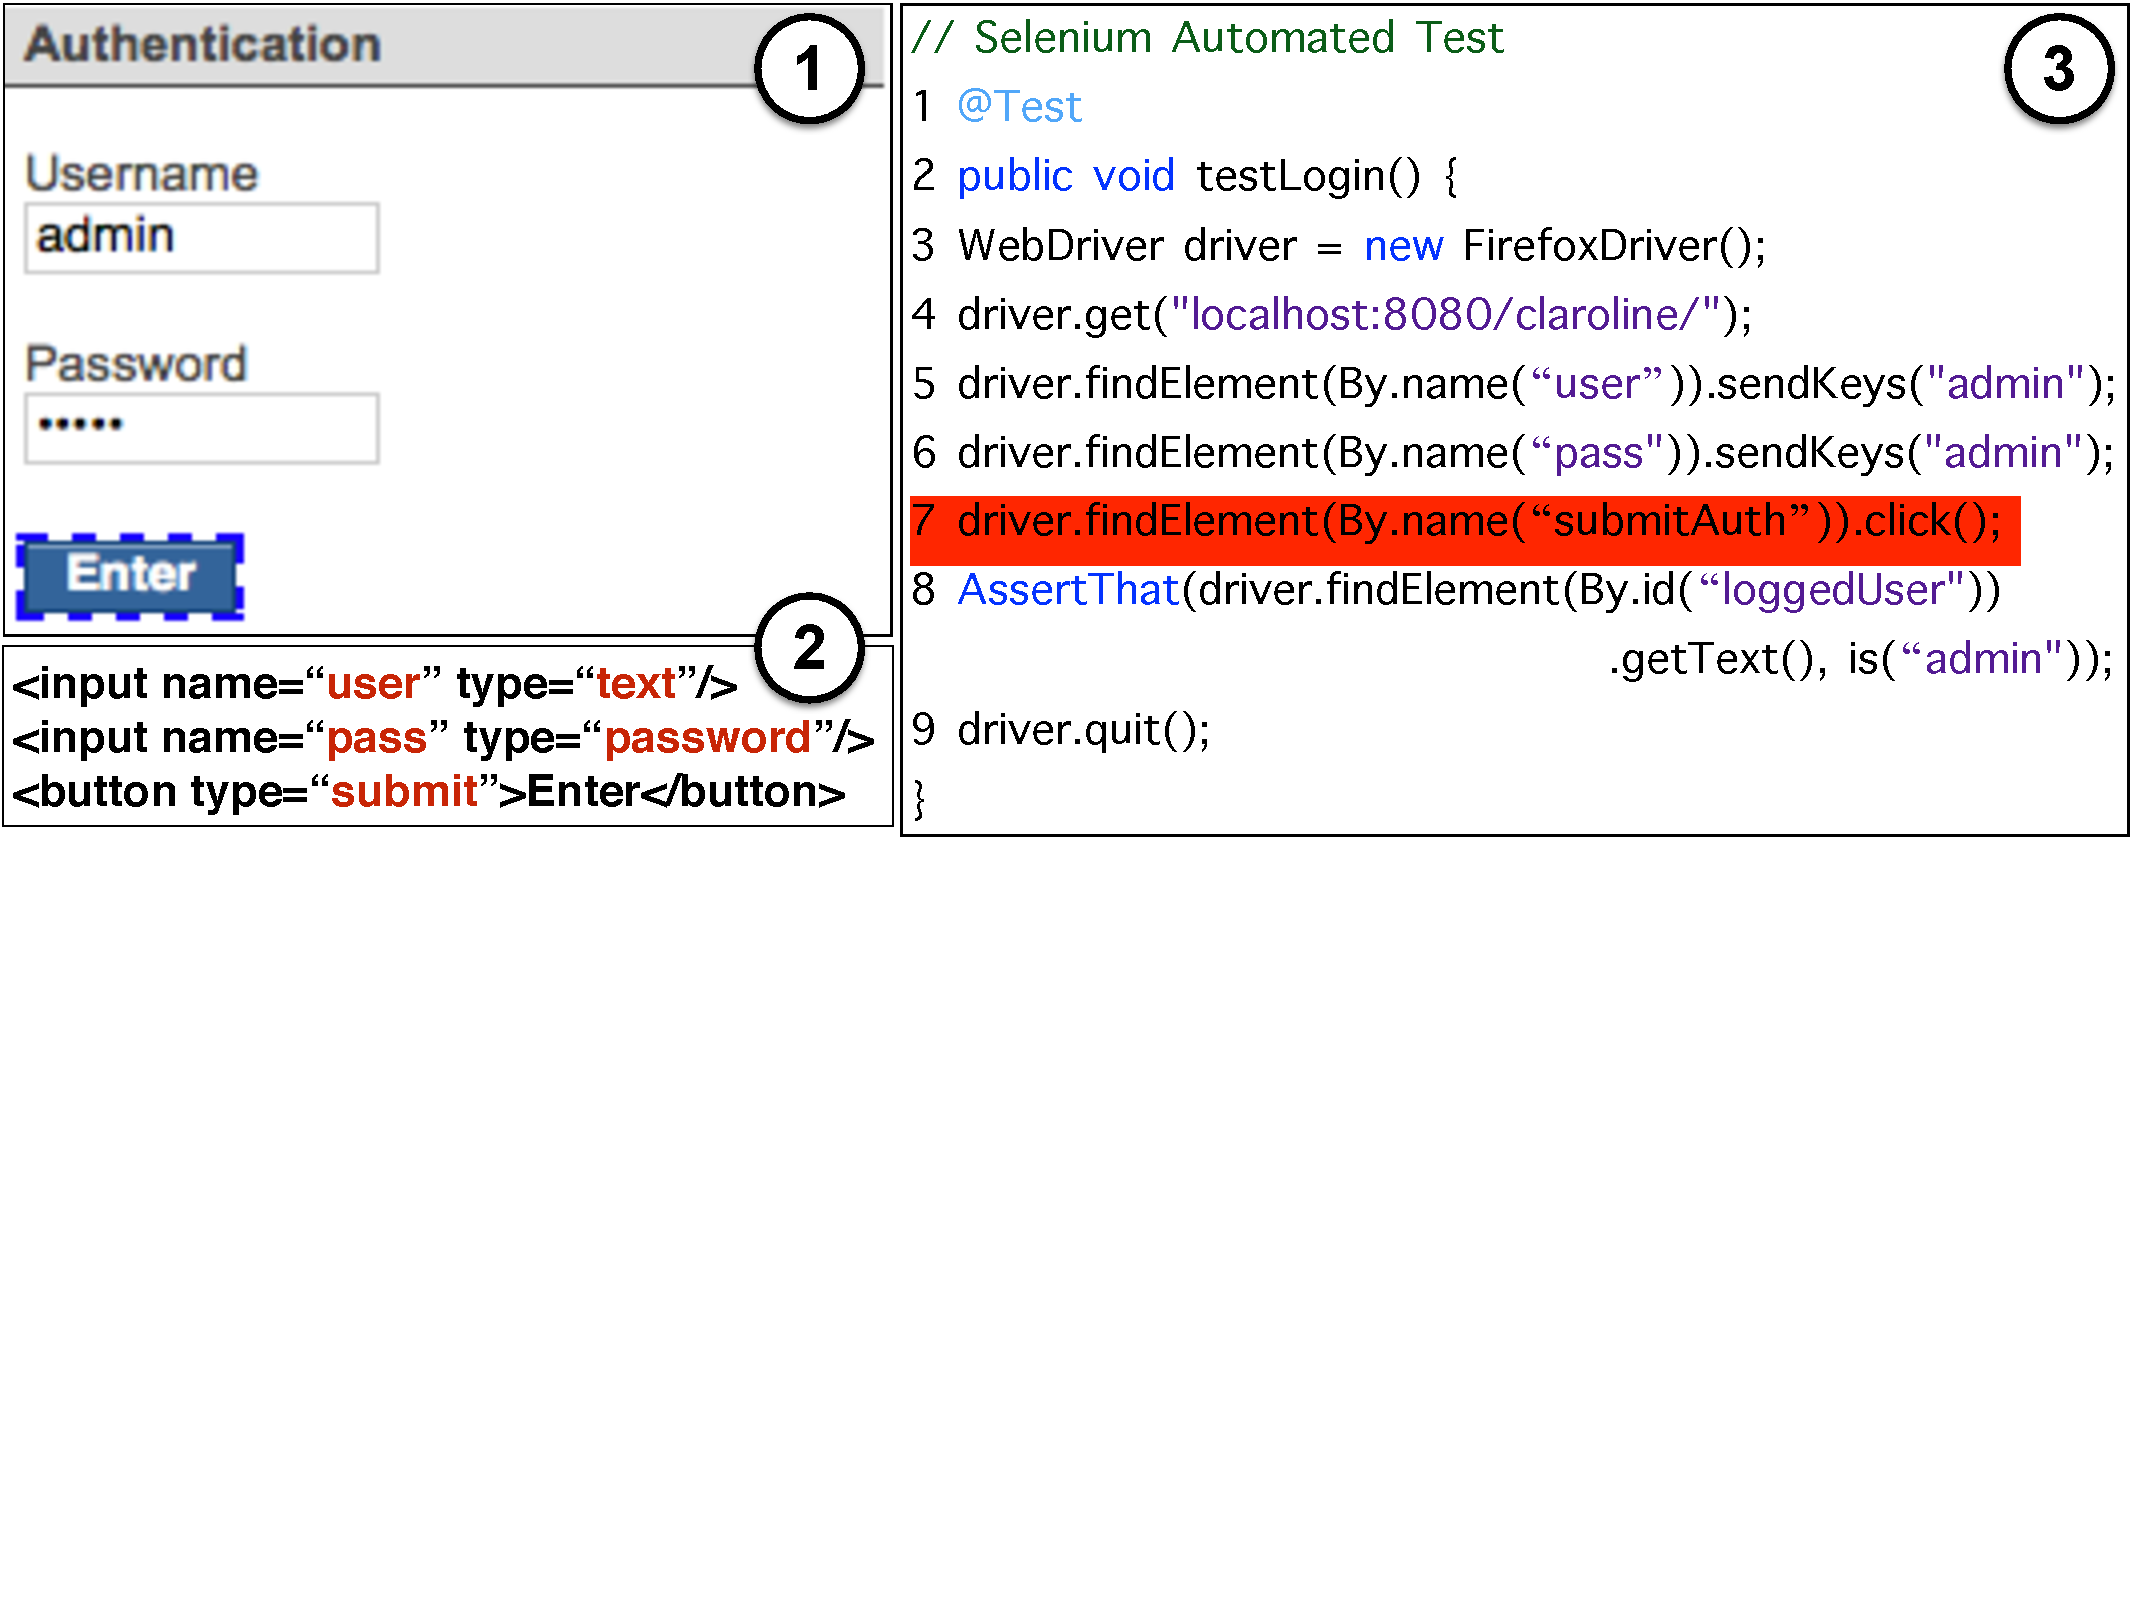
\includegraphics[trim={0cm 12.4cm 0cm 0cm},clip,scale=0.23]{images/claroline-version2}
%%}
%\caption{Login page of the Claroline web application (version 1.11.0), along with a portion of the corresponding HTML code, and an automated Selenium test}
%\label{claroline-version2}
%\end{figure}

\begin{figure}[t]
\centering
%\fbox{
%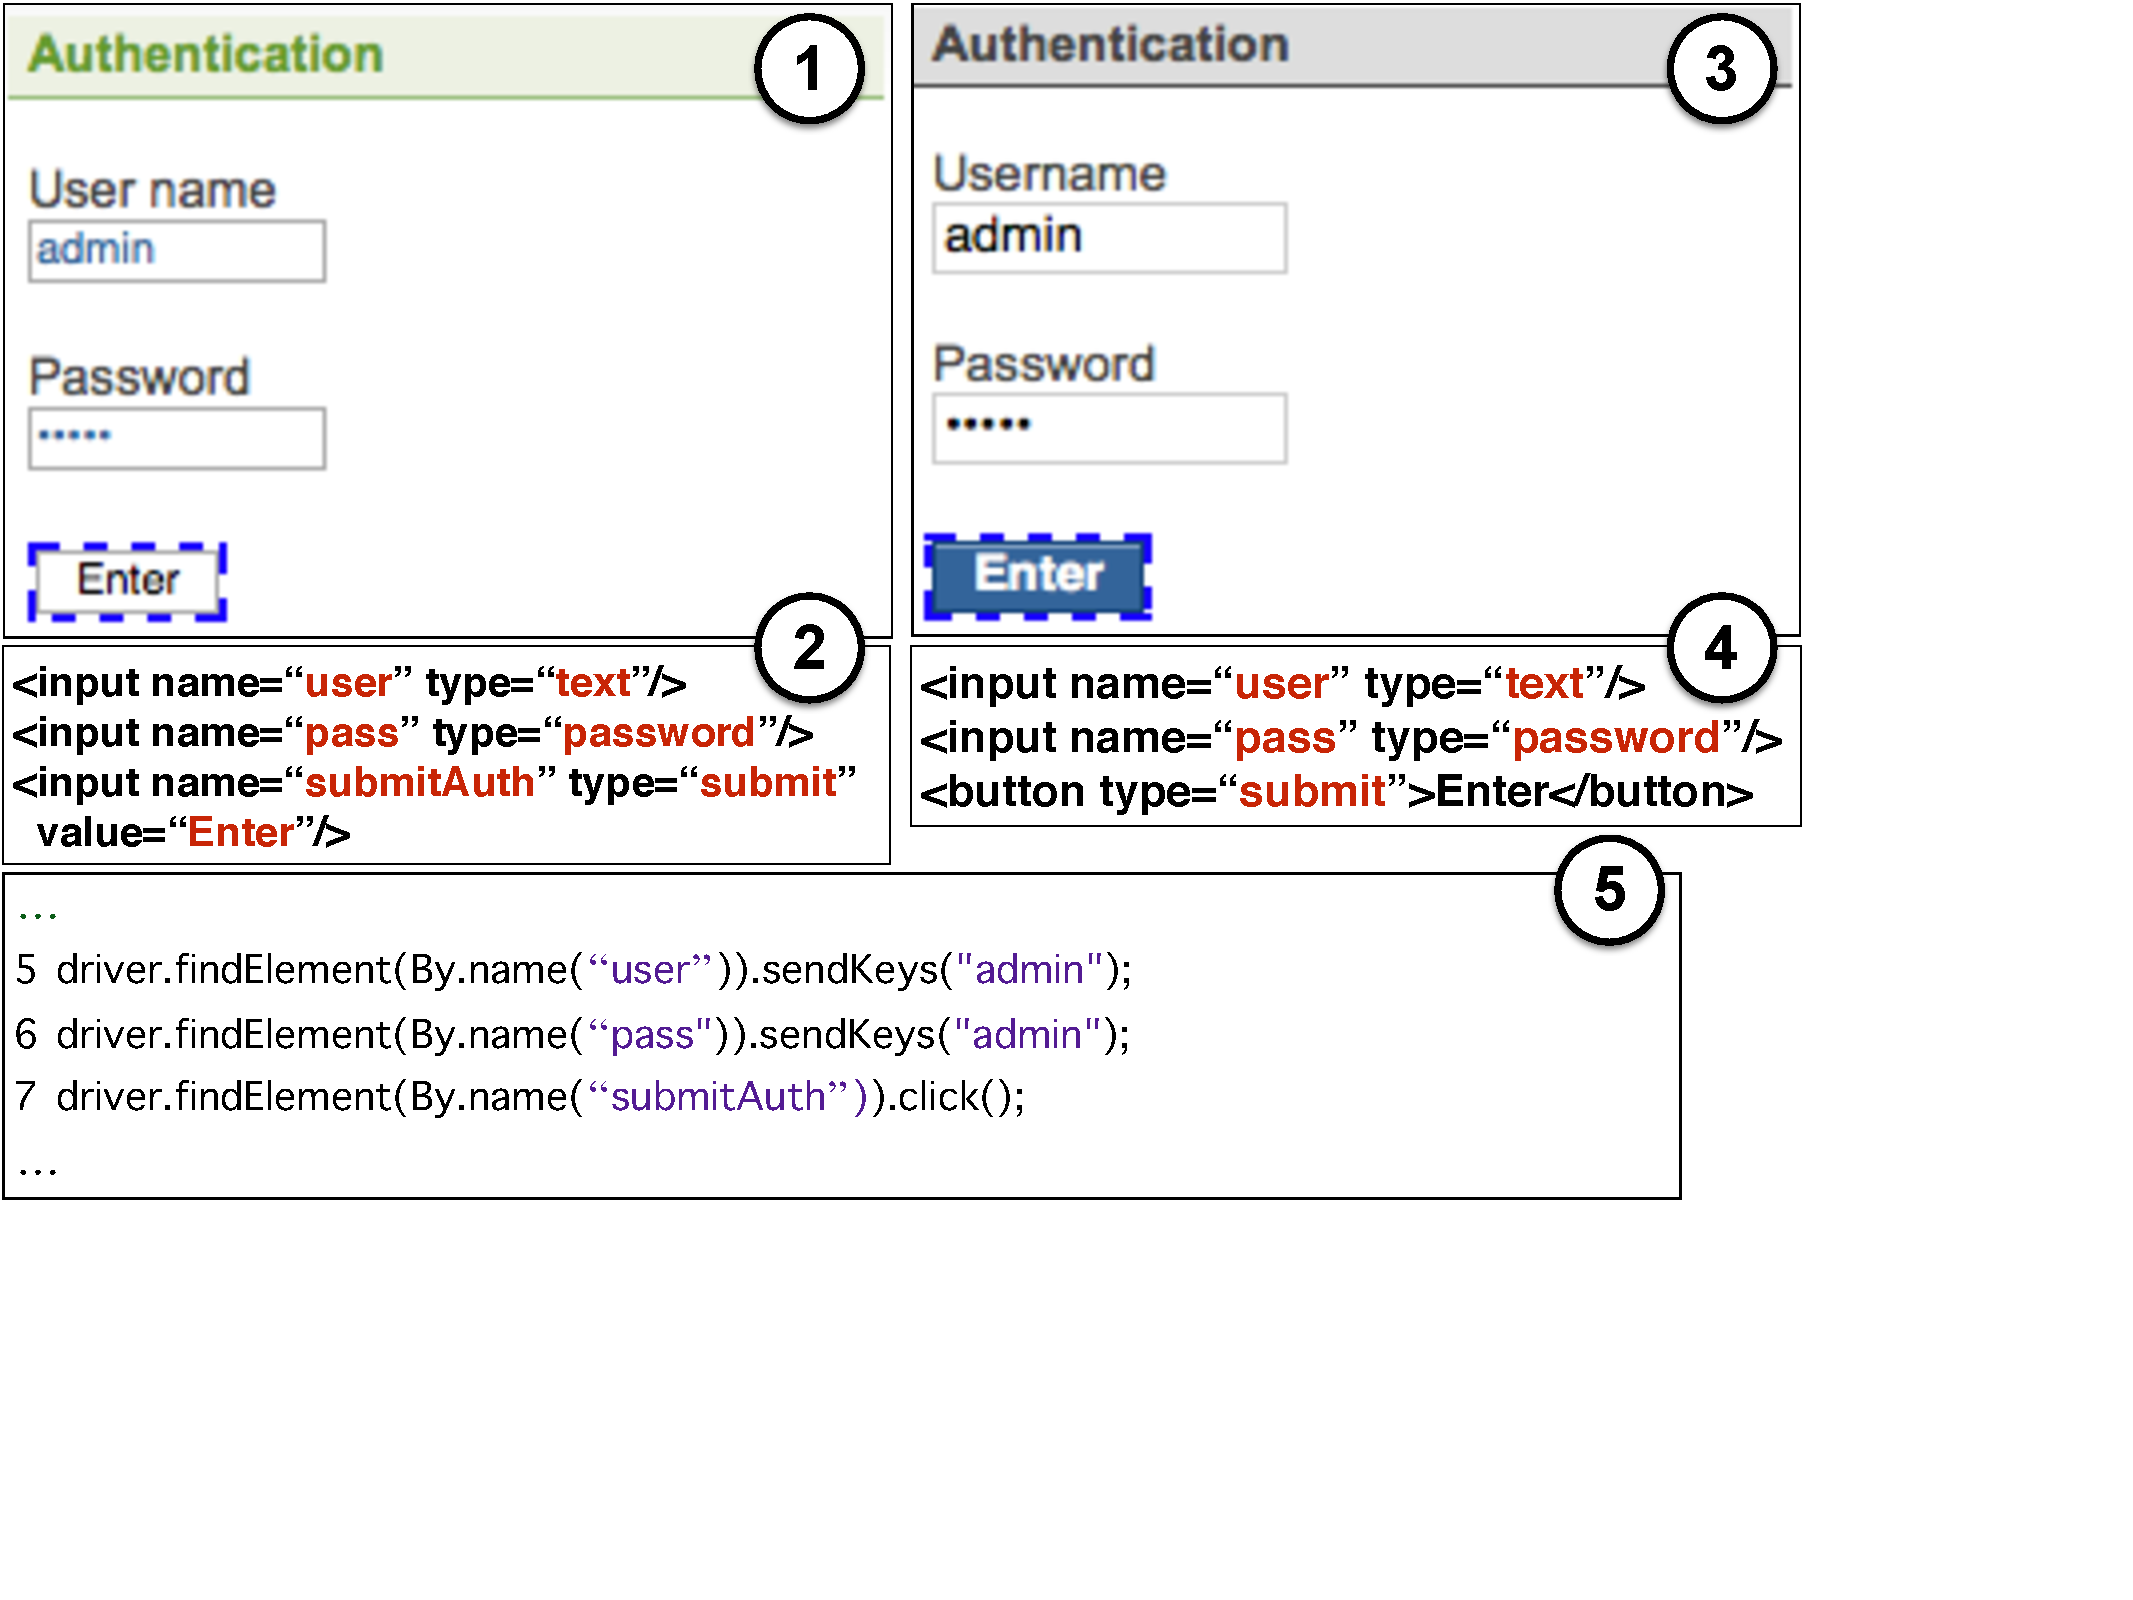
\includegraphics[trim={0cm 6.5cm 5.5cm 0cm},clip,scale=0.27]{images/claroline-together-2}
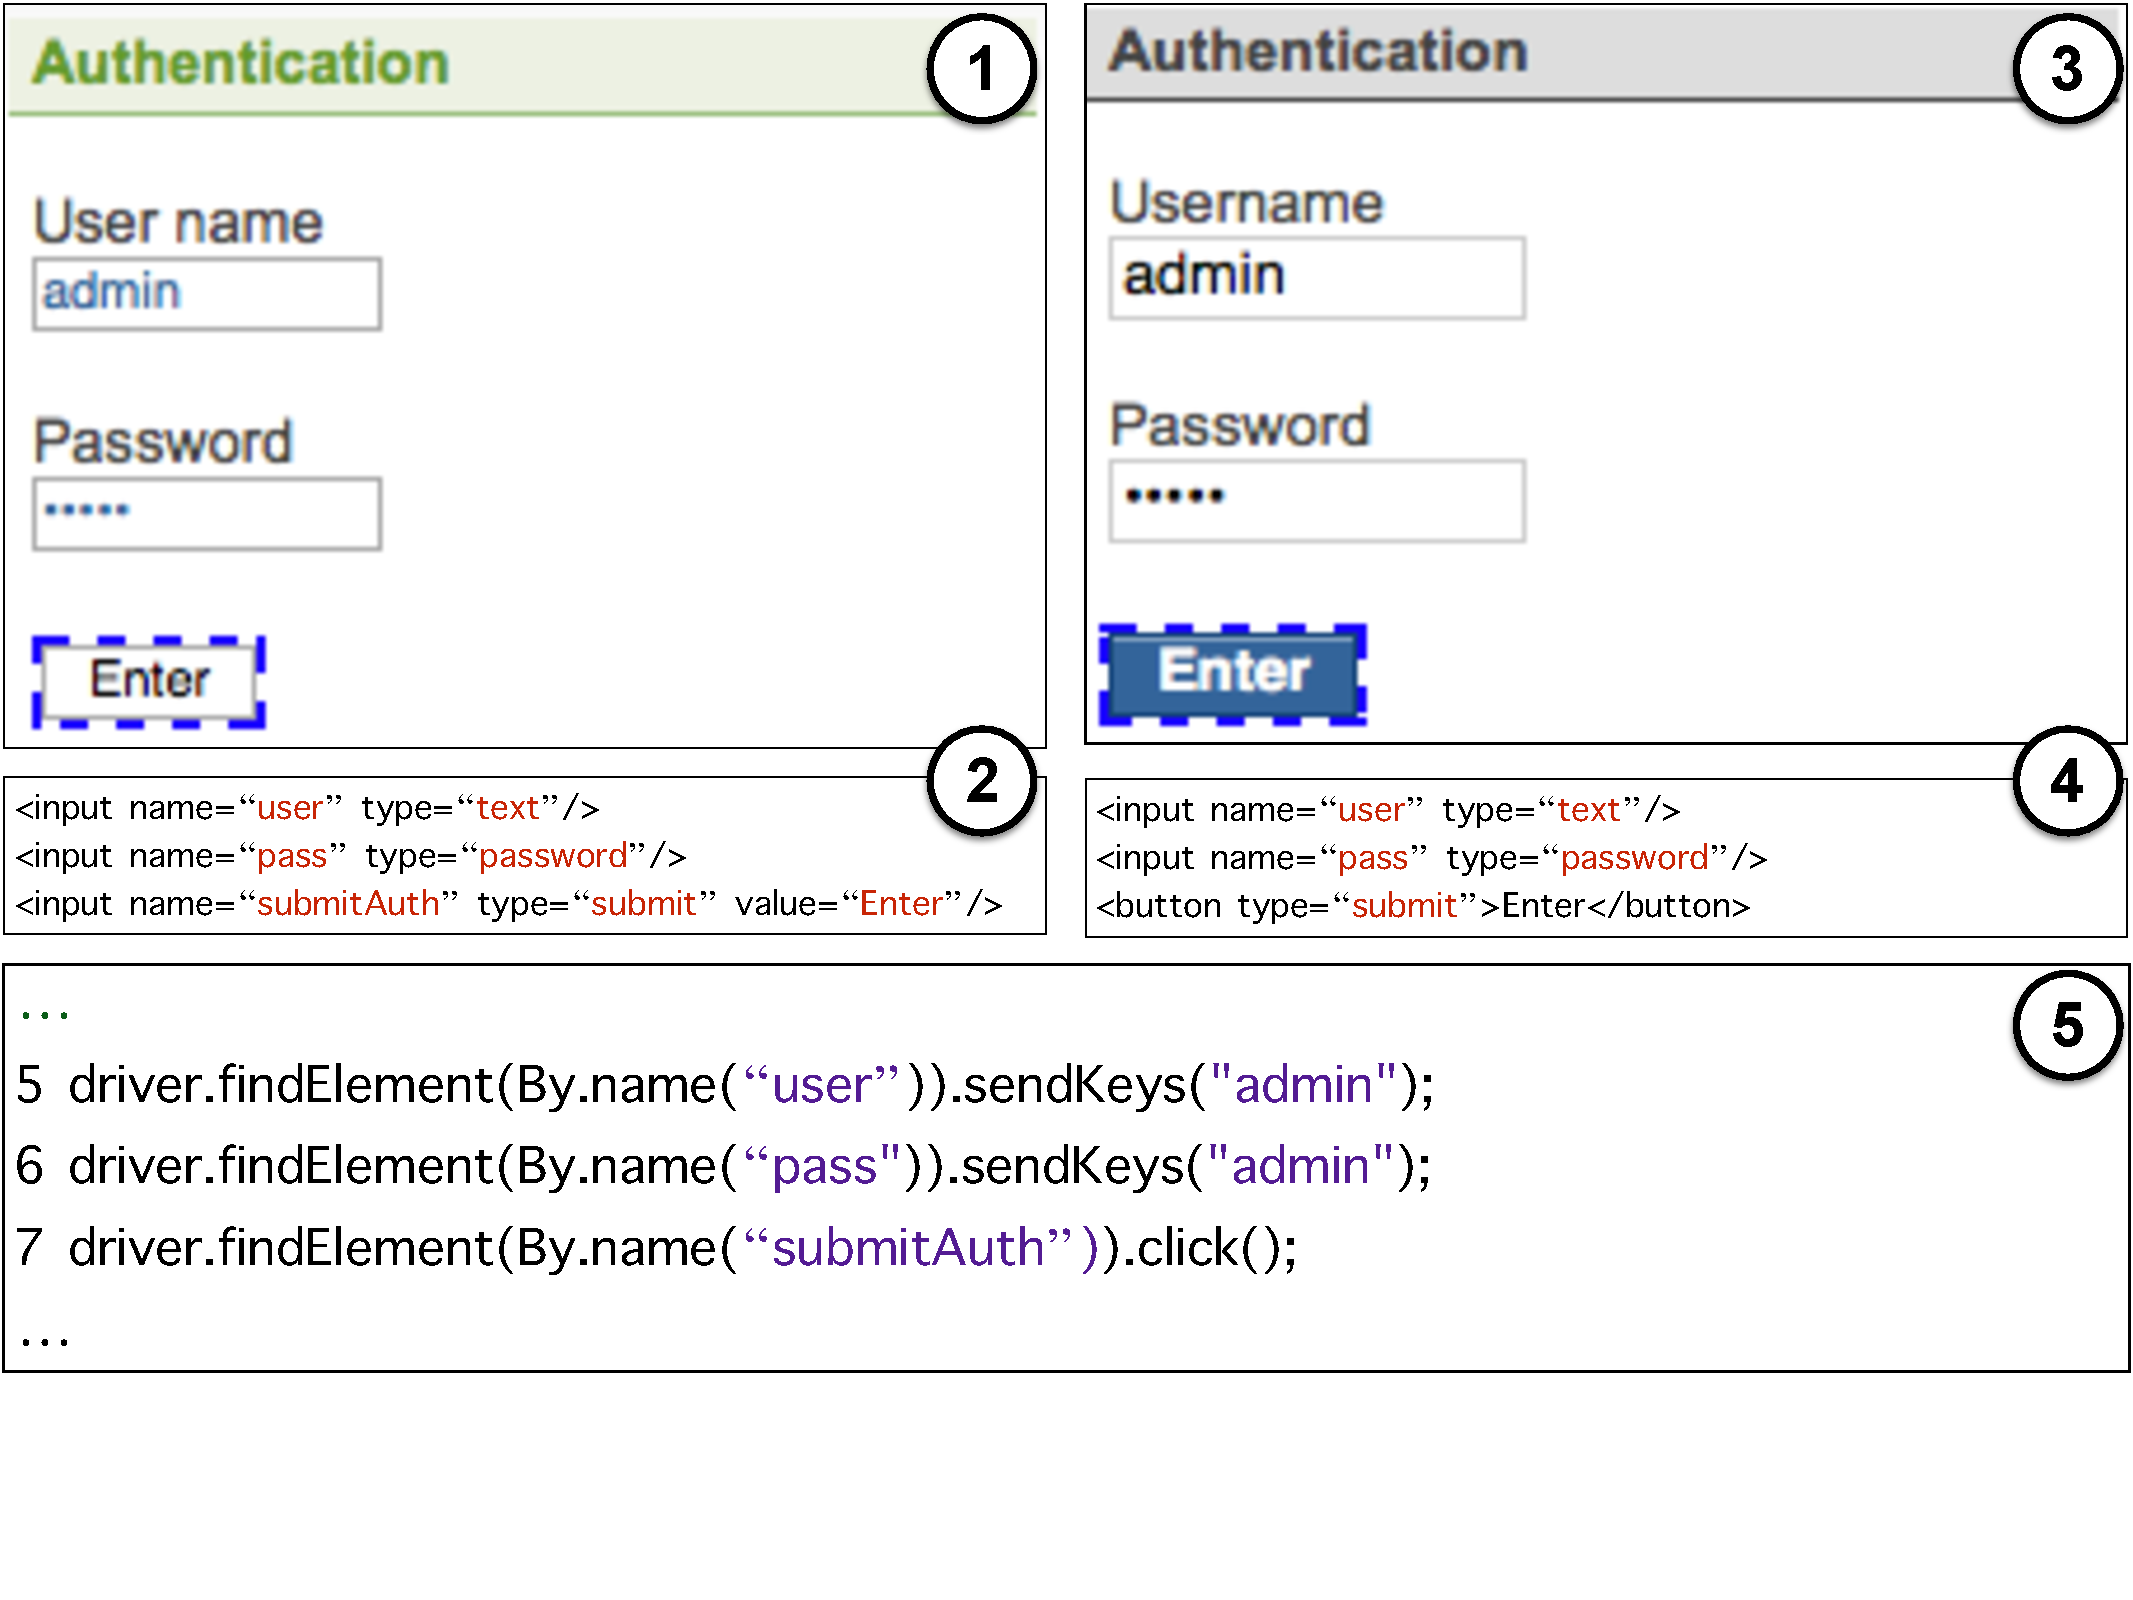
\includegraphics[trim={0cm 3.5cm 0cm 0cm},clip,scale=0.24]{images/claroline-together-3}
%}
\caption{Login page of the Claroline web application, version 1.10.0 (left) and 1.11.0 (right), along with a portion of the corresponding HTML code, and an automated Selenium WebDriver test}
\label{claroline-together}
\end{figure}

\subsection{Breakage Scenarios}\label{sec:breakage-scenarios}

Given the predominance of locator-related issues, we focus our analysis mostly on locator problems. In the following of this section, we present XXX\andrea{put number} challenging test breakage scenarios, and we show how the visual analysis can help to mitigate or correct such problems. However, we first formally define the concept of locator.

\begin{defn}[\textbf{Test statement}]
At a high level, each Selenium test statement is a tuple \textit{<locator, action, value>}.
\end{defn}

\begin{defn}[\textbf{Locator}] 
The locator component specifies the web element the test statement is interacting with. A locator is a function on a DOM state $D$. Notationally, $$l: D \rightarrow \{e\}$$ where $e$ is the web element returned by the locator $l$ when applied to $D$. 
\end{defn}

The locator function is surjective, that is every web element $e$ is mapped to by at least one locator (e.g., the XPath from the root to $e$), but there exist multiple locators {$\displaystyle \forall y\in Y,\exists x\in X{\text{ such that }}y=f(x).$} \andrea{stub. fix the definition}

\begin{defn}[\textbf{Action}]
The action component indicates either an event that is performed
on a web element during recording, or an action specific to Selenium's control of the replay.
\end{defn}

\begin{defn}[\textbf{Value}] The value component refers to any input entered by the test within the element specified by the locator.
\end{defn}

\subsection{Non-Selection}\label{sec:nonselection}

The first and perhaps most common scenario occurs when a locator $l$ applied to a certain DOM state $D$, returns no elements---formally, $l: D \rightarrow \emptyset$. 
%

\head{Scenario 1 (Non-Selection $\bullet$ Element Present)} 
Let us focus on the scenario in which the desired web element is still present on the page ($e \in D$). 
%To address this issue, first, a detection algorithm should make sure that $e \in D$. 
Then, possible repairs require to find another locator $l'$, such that $l': D \rightarrow e$.
This scenario is depicted in~\autoref{claroline-together}: \textcircled{\raisebox{-0.8pt}{1}}~shows the login form of Claroline web application version 1.10.0, together with the corresponding HTML code~\textcircled{\raisebox{-0.8pt}{2}}. \textcircled{\raisebox{-0.8pt}{3}}~shows the login form on the next major version of Claroline (1.11.0), and how the corresponding HTML code has evolved~\textcircled{\raisebox{-0.9pt}{4}}. 
%Let us a test scenario in which a user 
%inserts \texttt{username} and \texttt{password} 
%in the login form, and if these credentials are correct, 
%the \texttt{username} is displayed on the the homepage (not shown for brevity).
Finally, \autoref{claroline-together}~\textcircled{\raisebox{-0.9pt}{5}} shows a portion of a Selenium WebDriver test~\cite{selenium} which 
fills in the username and password input boxes (Lines~5-6), and submits the form (Line~7). Suppose the test was developed for (or evolved until) version 1.10.0, where it ran correctly.
%Line~8 verifies, by means of an assertion, the presence 
%of an HTML element containing the username in the home page, 
%and asserts that it equals the string ``admin''. 
%Finally, Line~9 shuts down the WebDriver instance 
%and closes the browser.

When executed on version 1.11.0~\textcircled{\raisebox{-0.8pt}{1}}, instead, the test will stop at Line~7, when attempting to locate the ``Enter'' button~\textcircled{\raisebox{-0.9pt}{3}}, because the attribute \mbox{\texttt{name="submitAuth"}} has been removed from the HTML~\textcircled{\raisebox{-0.9pt}{4}}. Typically non selection problems manifest as direct breakages, because the broken statement is the one that needs to be repaired.  
%
At a visual inspection of the two GUIs, a tester would expect the test to work, because her perception is immaterial where changes at DOM-level are concerned. Moreover, it is evident that the target element (i.e., the ``Enter'' button) is \textit{visually} still present on the page, and its position \textit{on the GUI} has not changed.
 
This is a simple instance of \textit{test breakage}, because the test scenario is unaltered, and no bugs are (eventually) present in the application. However, the automated test ceases to be applicable because it has lost the synchronization with the AUT, and a repair needs to be found.
At this aim, a tester may wish to use the \water  technique~\cite{Choudhary:2011:WWA:2002931.2002935} to automatically repair the broken statement at Line~7. Specifically, another locator for the ``Enter'' button~\textcircled{\raisebox{-0.9pt}{3}} needs to be found, rather the relying on ``broken'' attribute \texttt{name}. \water will attempt to gather information about the broken element (such as the XPath, and the various attributes) by analysing the DOM of the previous version 1.10.0, and match such information on the evolved DOM of version 1.11.0. Unfortunately, \water's technique is ineffective in such a scenario, because (1)~the attribute \texttt{name} has been deleted from the DOM, and (2)~the XPath and the tag of the target element have changed (from \mbox{\texttt{input}} to \mbox{\texttt{button}}), which renders impossible for \water's heuristic to identify it on the evolved DOM and apply its automatic repair.
%such as the XPath of the element, which is unfortunately inapplicable given that the tag of the element has changed (from \mbox{\texttt{input}} to \mbox{\texttt{button}}).
 
In this case, an algorithm taking into consideration the visual appearance of the test state might be able to match the target element between the two GUIs (in a similar way as a human tester would do). However, this task is challenging to be automated because several issues needs to be solved. Among all (1)~finding an accurate visual matching technique, and, in the case a visual match is found, (2)~retrieving the corresponding element in the DOM. \andrea{once all the scenarios will be described, this part might be refactored up}

\begin{figure*}[t]
\centering
\begin{subfigure}{\columnwidth}
\centering
%  \fbox{
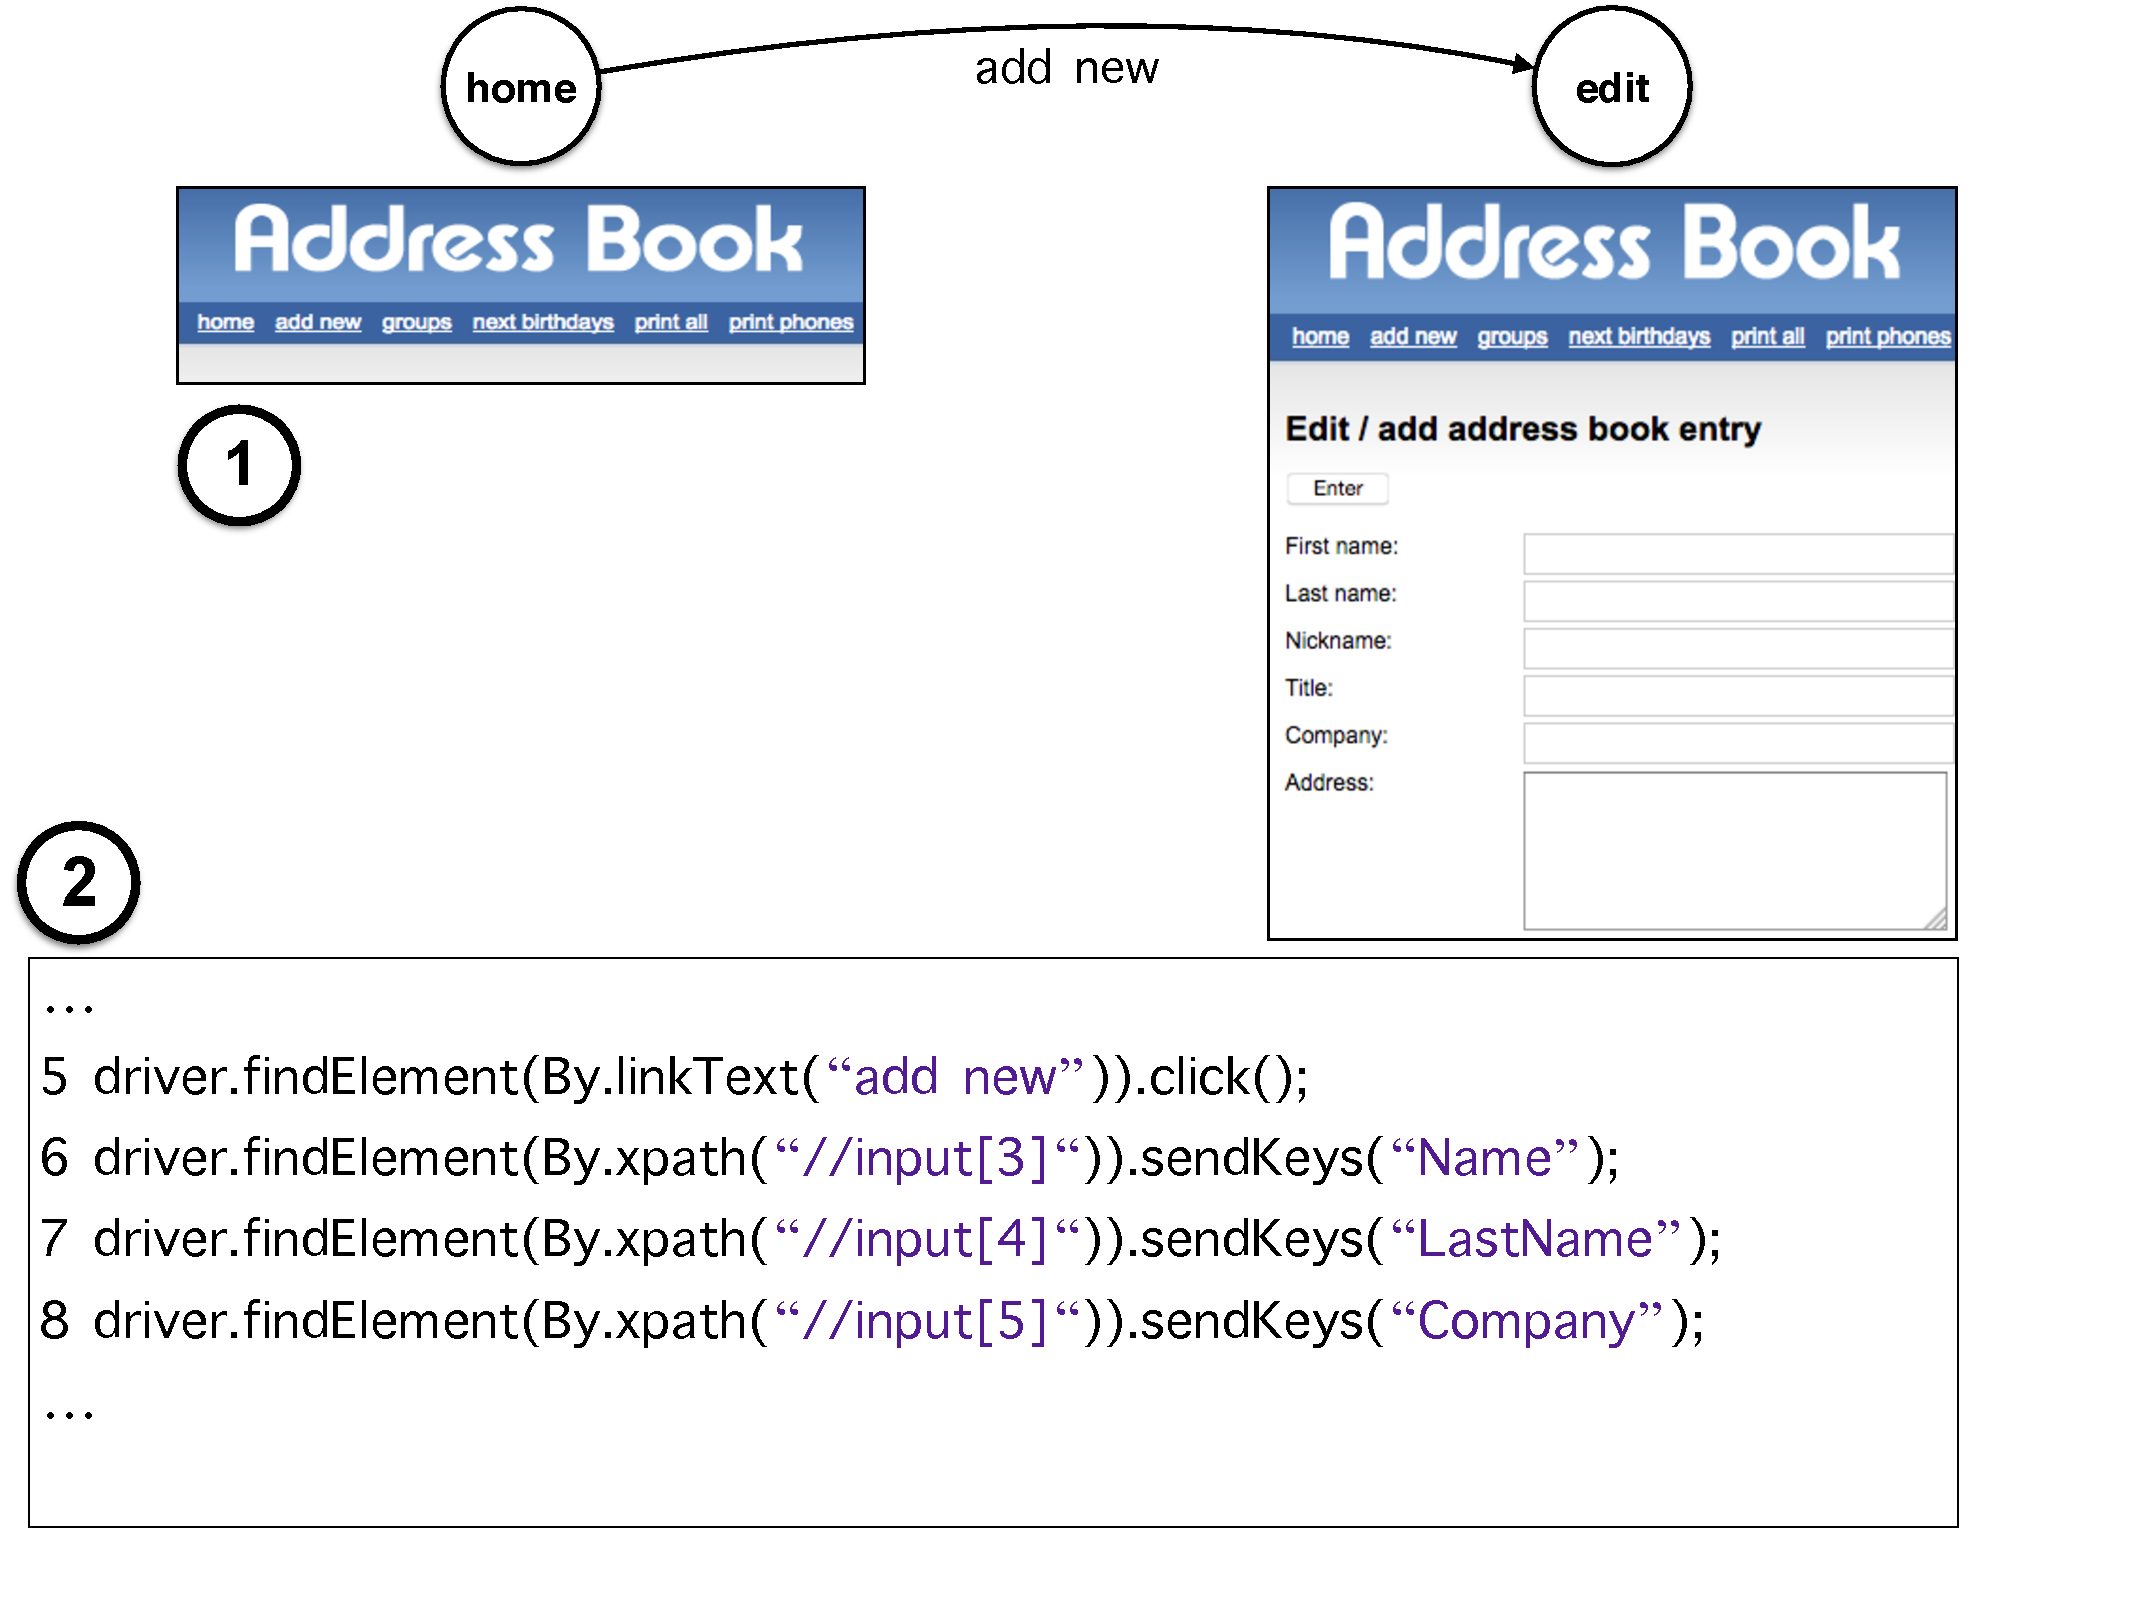
\includegraphics[trim=0cm 0cm 0cm 0cm, clip=true, scale=0.225]{images/misselection-part1.pdf}
%  }
\caption{\emph{Version 6.2.12}}
\label{fig:ab1} 
\end{subfigure}
\begin{subfigure}{\columnwidth}
\centering
%    \fbox{
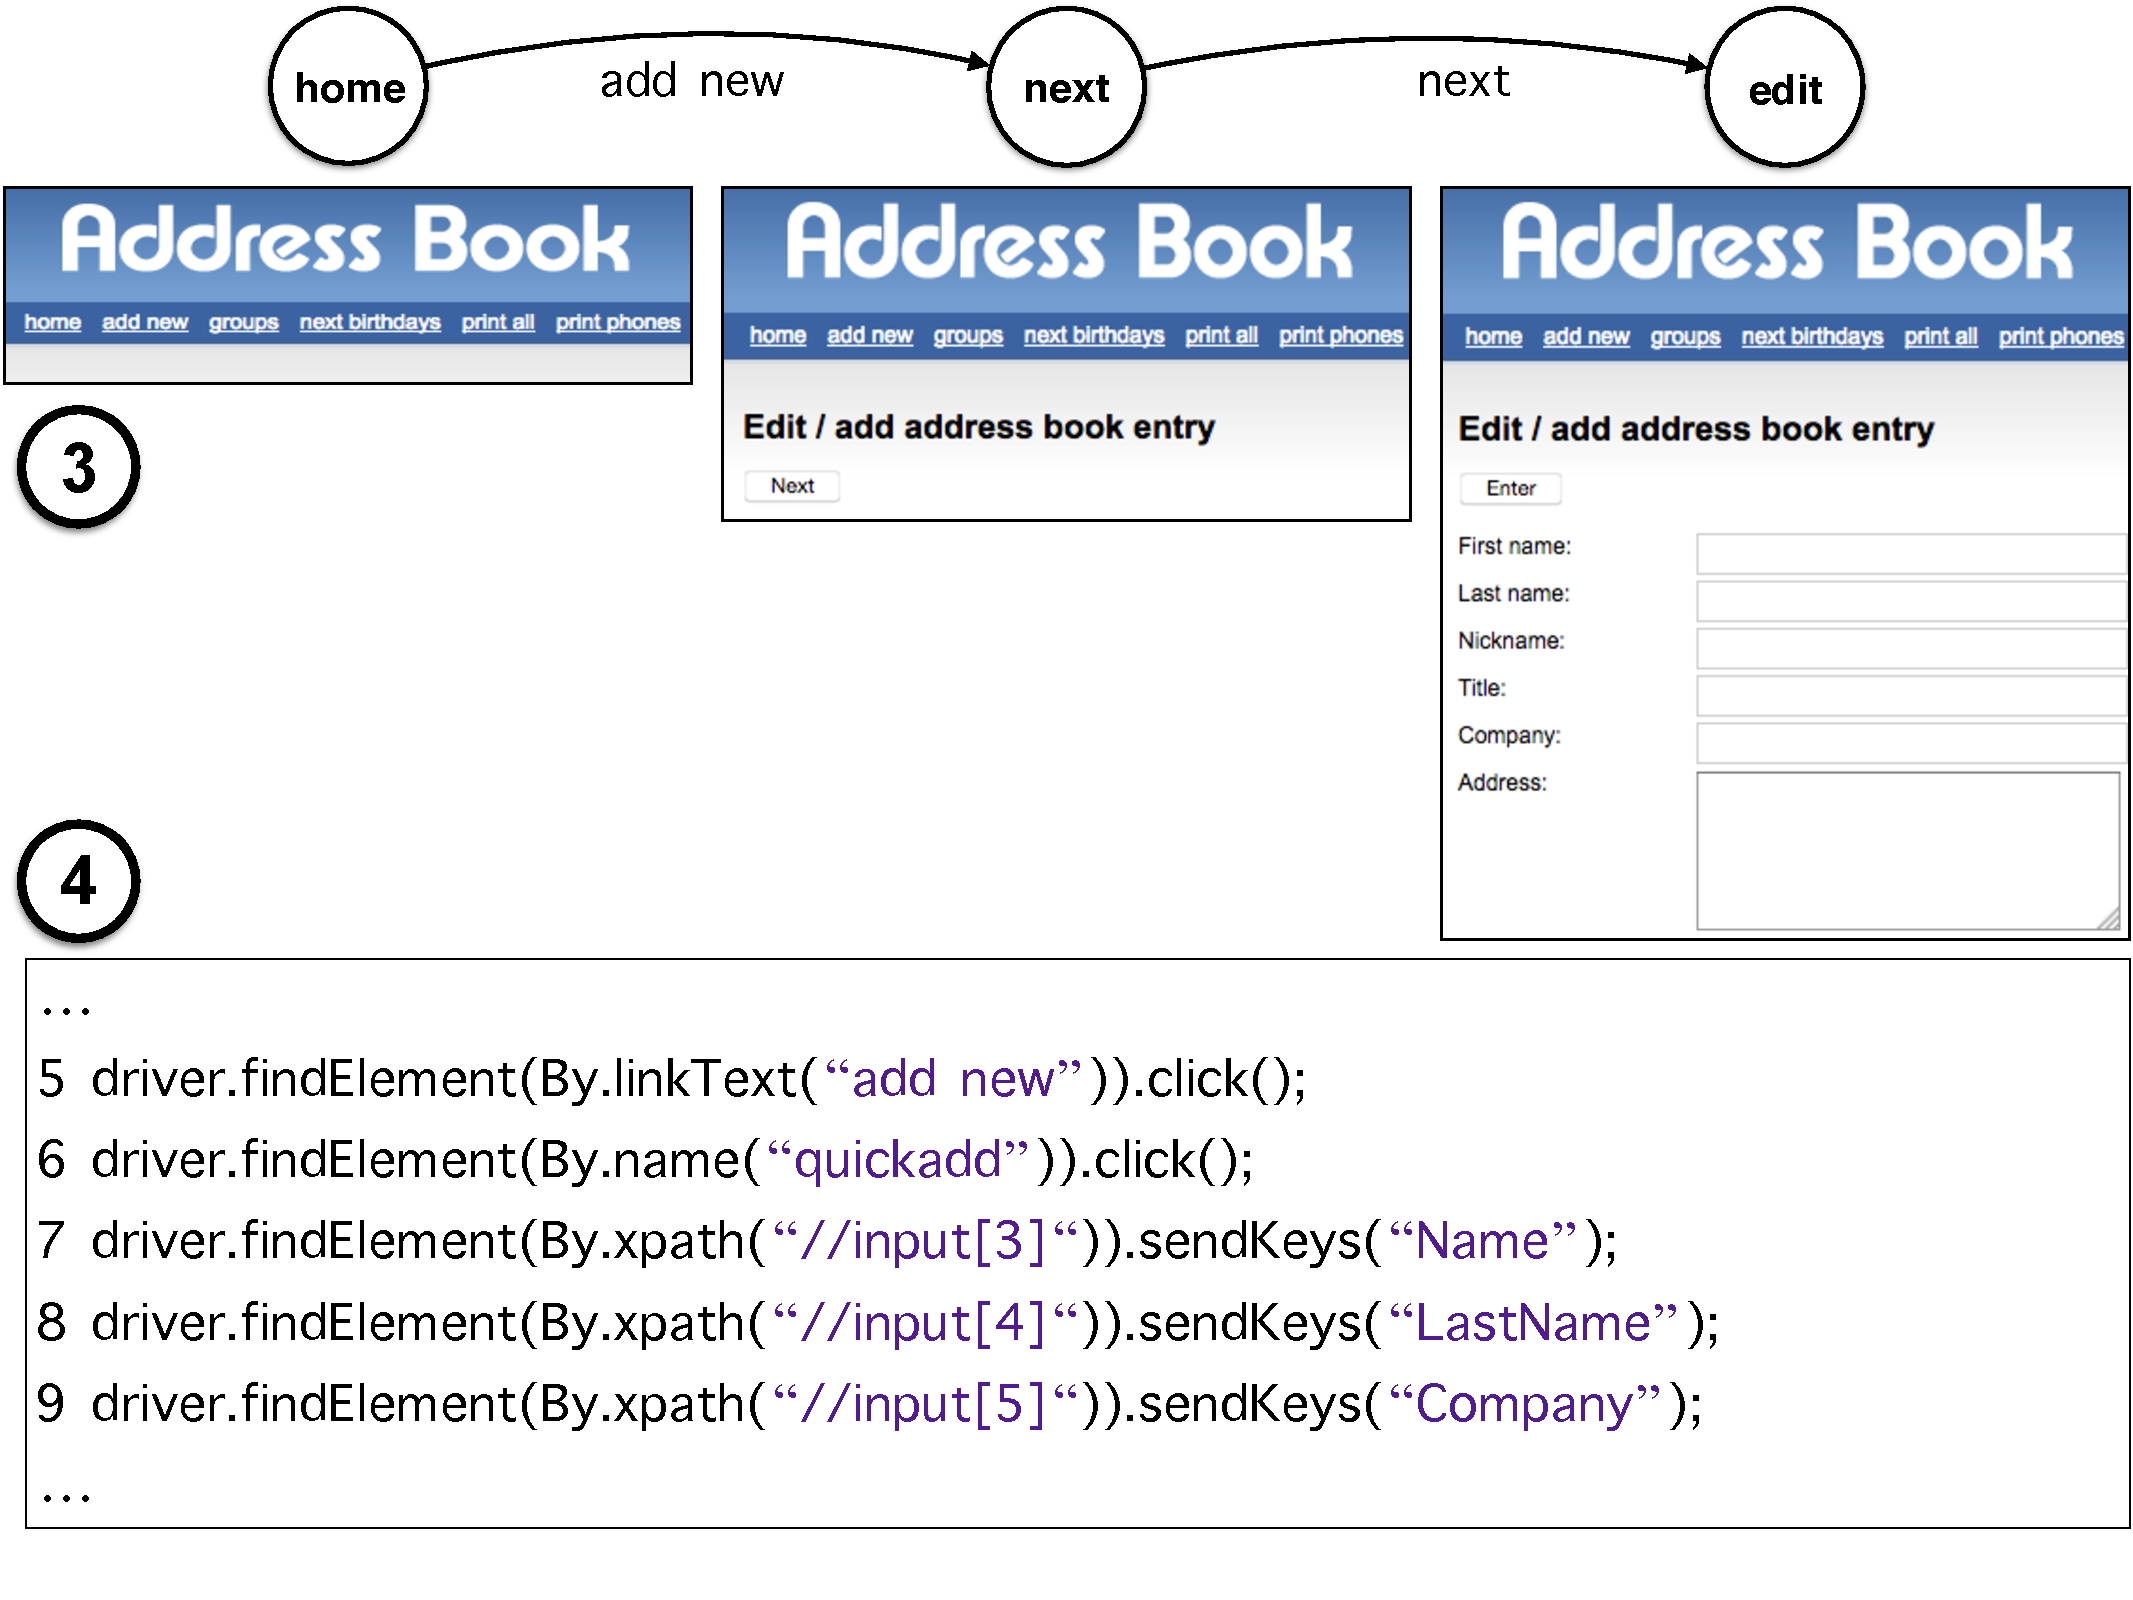
\includegraphics[trim=0cm 0cm 0cm 0cm, clip=true, scale=0.225]{images/misselection-part2.pdf}
%  }
\caption{\emph{Version 7.0.0}}
\label{fig:ab2} 
\end{subfigure}
\caption{AddressBook web application, version 6.2.12 (\ref{fig:ab1}) and version 7.0.0 (\ref{fig:ab2}), along with a portion of the navigational graphs, and automated Selenium WebDriver tests}
\label{misselection}
\end{figure*}

\noindent
\textbf{Scenario 2 (Propagated) or Non Selection Neighbouring State.} 
As a concrete example consider \autoref{fig:ab1}, showing Addressbook web application version 6.2.12~\textcircled{\raisebox{-0.7pt}{1}}, specifically the pages in which the user can insert a new entry. The test~\textcircled{\raisebox{-0.7pt}{2}} clicks on the ``add new'' link on the home page (Line~5), and fills in the First name, Last name and Company text fields (Lines~6--8).
Suppose now to replay the test on the successive version 7.0.0~\textcircled{\raisebox{-0.7pt}{3}}, for regression purposes. The test will raise an exception of kind \texttt{NoSuchElementException} at Line~6, when attempting to locate the ``First name'' text field~\textcircled{\raisebox{-0.7pt}{2}}. 
Indeed, a new intermediate confirmation page has been added~\textcircled{\raisebox{-0.9pt}{3}}, and the navigational workflow of the test must be corrected to reflect that of the new modified web application.

From a tester perspective, the ``First name'' text field can no longer be found in the web page (test state) following the execution of the statement at Line~5. However, conceptually, the repair action that needs to be triggered in order to correct the test has nothing to do with the locator at Line~6.
In fact, by only looking at the exception raised by JUnit, it is  challenging for the tester to detect this problem, unless the \textit{visual execution} of the test is taken into consideration.
%
Even the use of \water~\cite{Choudhary:2011:WWA:2002931.2002935} is unsuccessful, because it would attempt at repairing the broken statement at Line~6. (the technique only handles addition of statements within forms, and does not apply to general broken workflow scenarios).

In order to address this issue, we need to (1)~identify that the target state following the execution of a statement $st_i$ has changed between the two versions, (2)~mapping the web element $e \in st_i$ in version $V$ onto $st_j$, i.e., a neighbouring state of $st_i$  in the new version $V'$, which requires to (3)~finding  a web element $e' \in st_i$ such that $(e', st_i) \rightarrow st_j$ (the ``Next'' button in our example~\textcircled{\raisebox{-0.7pt}{3}}).

\noindent
\textbf{Scenario 3 (Non-Selection $\bullet$ Element Removed).} 

\subsection{Mis-Selection}\label{sec:misselection}
Problems occur not only when web elements are being deleted, but also when they get modified, either in their position on the DOM tree, or their position in the application state space. This can cause tests to ``mis-select'' elements, which is another breakage scenario we aim to address.

Specifically, a mis-selection occurs when a locator selects a different DOM element from the one that was used to target. Suppose having version $V$ and a test $t$, composed of a statement $st_i$, which uses a locator $l$ (where $l: D \rightarrow \{e\}$).
In the next version $V'$, $l: D' \rightarrow \{e'\}$ where $e \ne e'$.
A mis-selection of an element can lead to unpredictable misbehaviours of the test. In the following of this paragraph we analize two scenarios pertaining to mis-selection problems. 
%In the following of this paragraph we analize two scenarios: (1)~the execution of a statement $st_i$ is supposed to trigger a certain state transition. Due to the mis-selection of the locator contained $st_i$, the transition does not take place (i.e., the app remains in the same state), and a later statement $st_k$ (with $k>i$) breaks. (2)~the execution of a statement $st_i$ triggers an unexpected state transition, that makes a successive statement $st_k$ (with $k>i$) to break (propagated).

\noindent
\textbf{Scenario 3 (Mis-Selection (Direct)).} 
Consider \autoref{misselection} again. 
Suppose that the test~\textcircled{\raisebox{-0.9pt}{2}} is repaired so as to reach the edit page on version 7.0.0 (for instance, a click on the Next button has been added between Line~5 and Line~6). On the new version 7.0.0, the statements at Lines~6--7 will execute correctly, whereas the statement at Line~8 will fill the field Nickname, instead of the field Company. In the literature, this is known as mis-selection problem~\cite{Choudhary:2011:WWA:2002931.2002935}, formally, $l: D \rightarrow e'$ where $e \ne e'$. The mis-selection problem leads to unpredictable test executions, that diverge from the test's intended behaviour. Depending on the kind of actions, the test execution might result in a propagated or a silent breakage~\cite{Hammoudi-2016-ICST}. A propagated breakage occurs when the test breaks in a different point from the one in which the breakage originates. Typically, the test continues its execution until it reaches a point in which an action cannot be performed or an element cannot be found, but the actual repair has to be triggered \textit{in a previous test statement}. Once again, those scenarios are challenging to discover for the tester, because only at a careful manual inspection of the test execution, one can recognize such breakages patterns.

%\andrea{this kind of breakage is associated mostly to XPath locators, but it can happen with attributes too if, for instance, two different elements share the same attribute locator.}

\head{Summary}
In this section, we have presented XXX \andrea{put number}  test breakage scenarios and we have shown how the visual appearance of the SUT can be utilized to overcome the existing test repair approaches and give an important contribution to the tester. We do not claim, however, that such a list represents all the possible scenarios. Note that the presented scenarios might (1)~occur together (i.e., leading to \textit{multiple} breakages in the same test) or (2)~interleave with each other.\andrea{is that possible possible?}

%\begin{figure}[t]
%\centering
%%\fbox{
%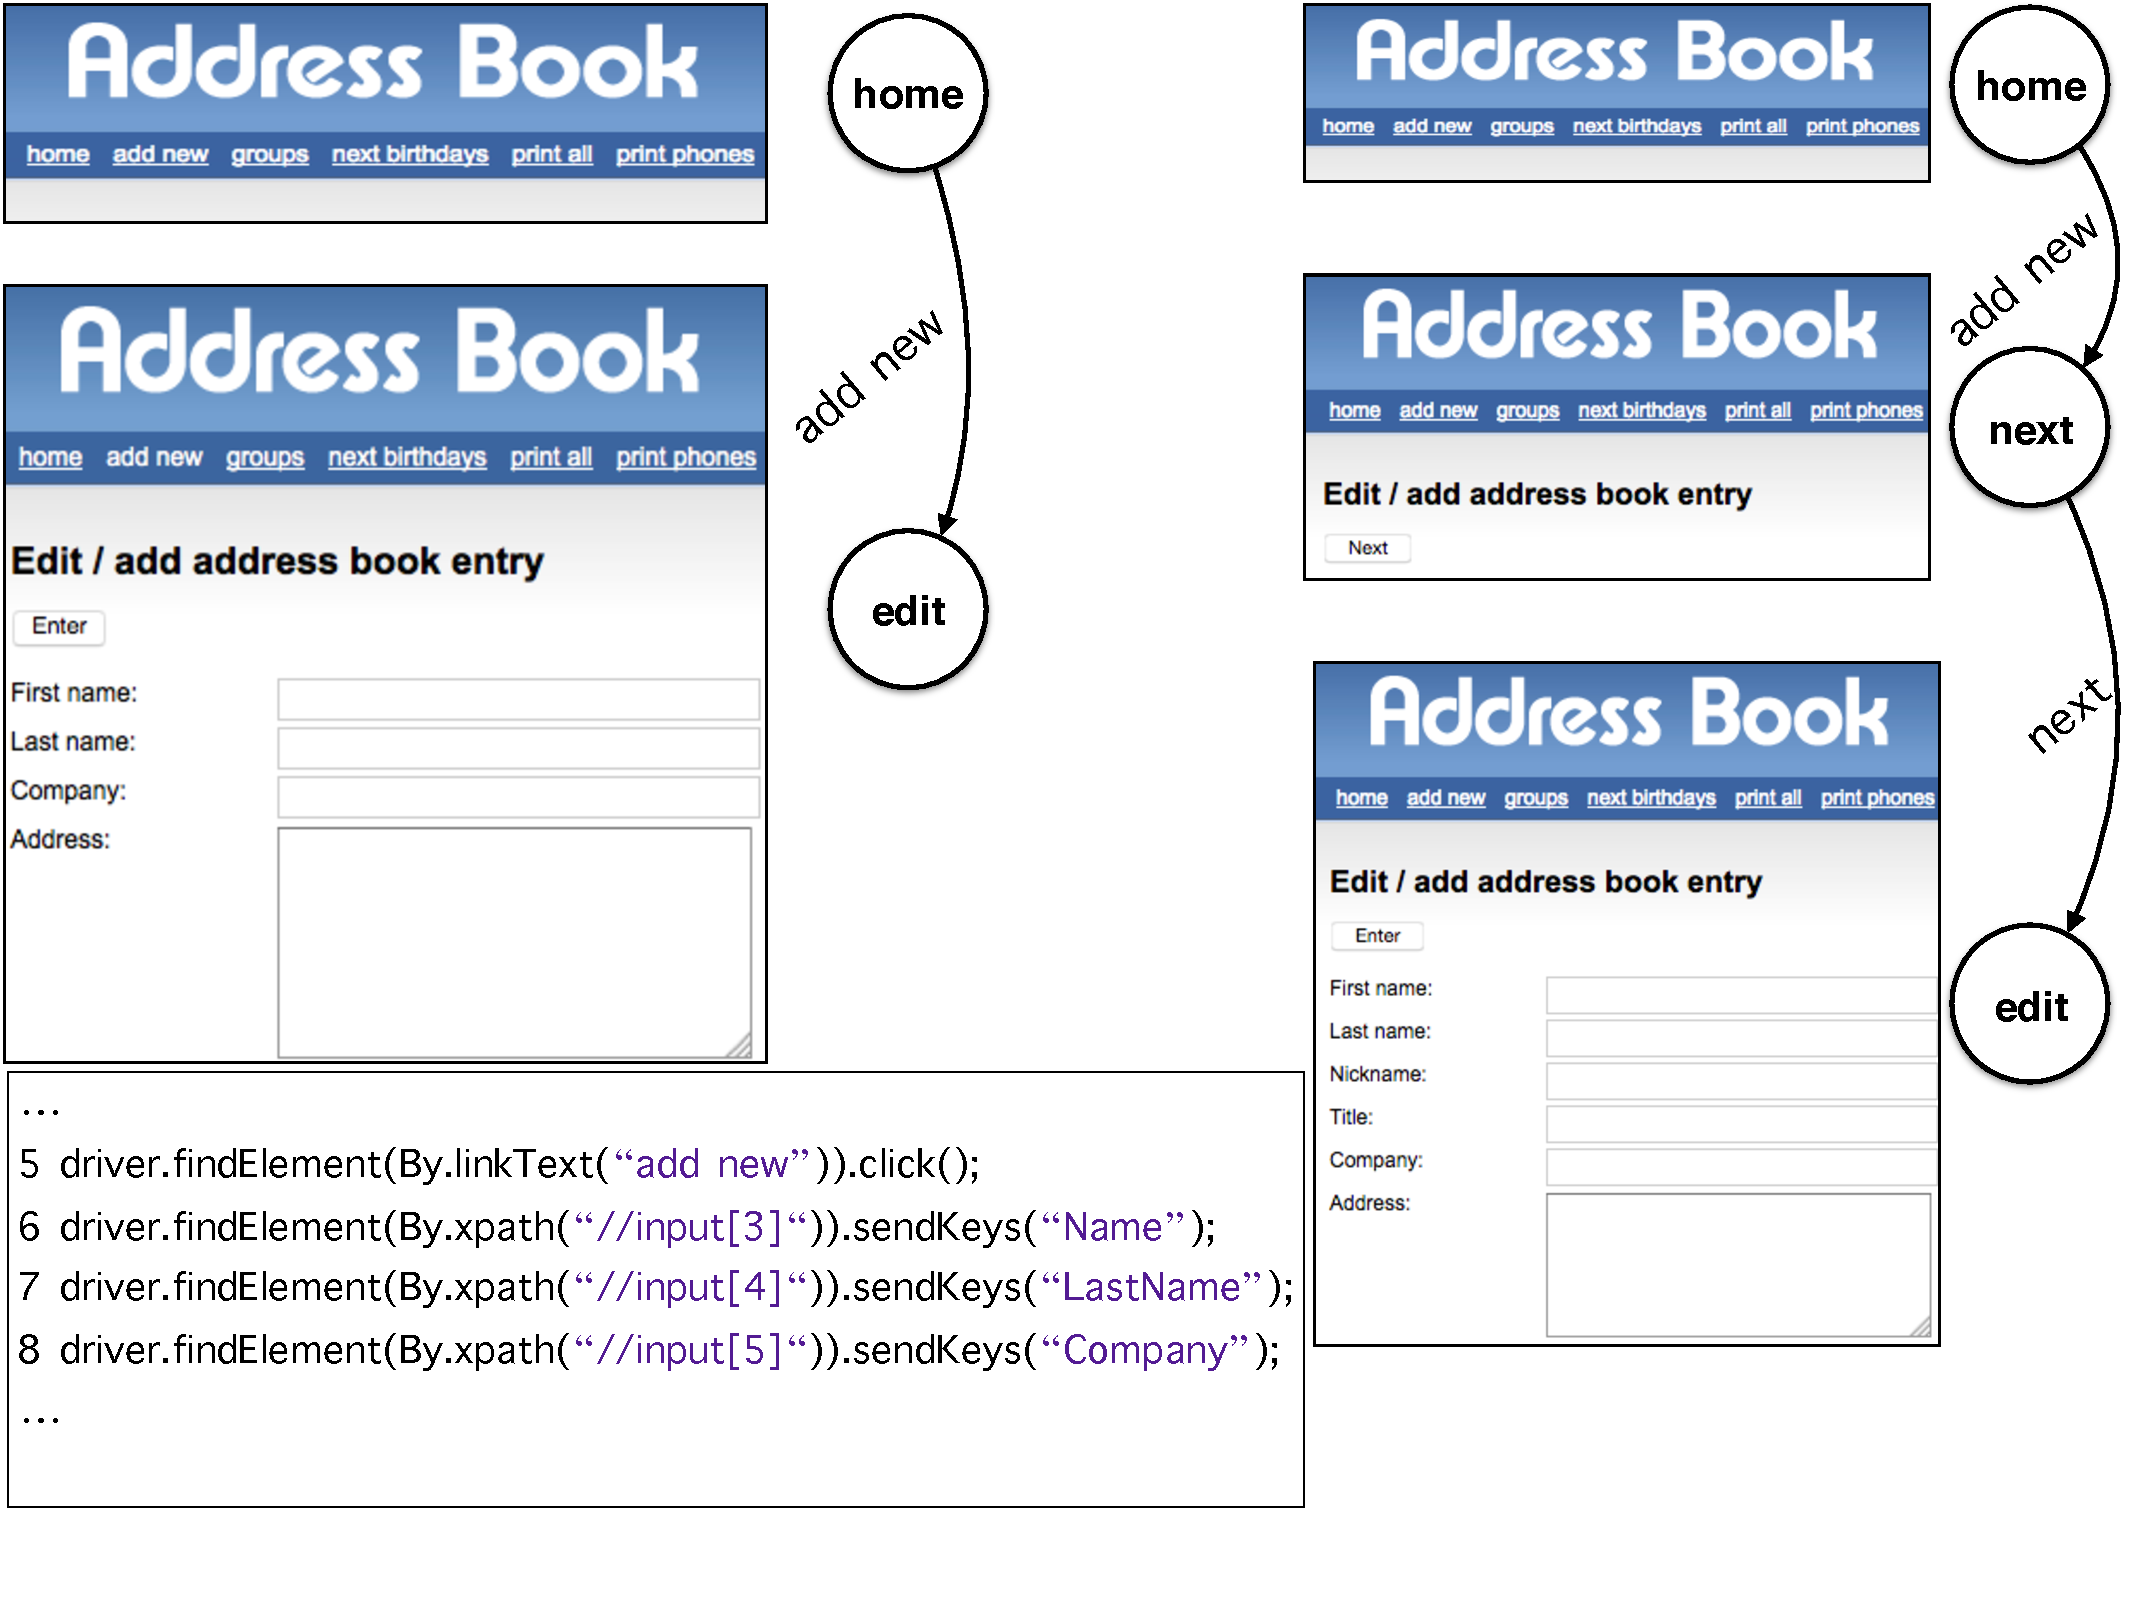
\includegraphics[trim={0cm 1cm 0cm 0cm},clip,scale=0.23]{images/misselection}
%%}
%\caption{Examples of mis-selection}
%\label{misselection}
%\end{figure}

\subsection{How Testers Repair}

When a test $t$ that was used to function on a version $V$  breaks on a successive version $V'$, a tester needs to understand the root cause behind the breakage and a possible repair for it. 

In doing so, at least four steps are involved: 
(1)~the tester inspects the error stack trace or the console, which may contain information about the origin of breakage (e.g., ``\texttt{NoSuchElementException} occurred. Unable to locate element with \mbox{\texttt{name=password}}''). 
(2)~the tester inspects $t$ to find the statement $st$ responsible for the failure; %which is also likely to be the one that needs to be corrected (note that this is not always true).
(3)~the tester navigates the GUI of $V'$, trying to identify the portion of the GUI which is related to $st$. 
(4)~depending on the kind of breakage, the tester inspects either the (i)~DOM of $V'$, or (ii)~the GUI of $V'$, or (iii)~both the DOM and the GUI, to find candidate repair solutions. In doing so, the tester may possibly need to exercise manually the same broken scenario of $t$ (i.e., all the actions in the statements preceding $st$), in order to replicate the breakage occurred at $st$ and gather insights on possible repair actions.

To wrap up, a \textbf{first challenge} in repairing web tests derives from the fact that  
%Thus, in E2E web tests such as Selenium's 
the tester often needs to inspect and link the behaviour of the test code execution, along with the modification perpetrated to the GUI and the DOM of the application. 
In other words, breakages are often repaired by finding candidate solutions through the inspection of the DOM and the GUI \textit{at the same time}.
For this reason, it is arguably more difficult (or more time consuming) to repair Selenium's tests than standard JUnit tests for desktop applications (for which the error messages are typically more informative and IDE features make the debugging activities easier).

A \textbf{second challenge} is related to the time needed to find and correct the breakages, which may be significantly high~\cite{Leotta-TAIC-2013,JAMAICA2013}. One of the main reasons is due to the low support by the existing test automation tools in understanding the root causes behind test breakages and how they do relate with the changes made in the web applications. 

In this paper we wish to make step ahead to provide such understanding. 
Our aim is to combine the knowledge present in the DOM of the application with its visual appearance, so as to effectively aid the tester in the test repair problem. Our approach aims at automating the mental model the testers create when a test case is executed against a web application GUI. In our belief, such a model is a viable means for automating test case repair.

Existing locator repair techniques are indeed limited when the web application undergoes drastic structural changes because they only consider the DOM as source where to find possible repairs.
However, we argue that visual image recognition can help to fix all the breakages that pertain to ineffective locators that target web elements that are still present and visually displayed within the same web page.

\subsection{Computer Vision Stuff}

\subsection{General Terms}

In object detection problems we usually have two sets of images. The training set is used for showing the computer what the desired object looks like. This can be done by calculating hue histograms or by computing keypoints and keypoint descriptors. Obviously, it is preferable that training images are either annotated (locations of objects of interest are specified by bounding boxes) or just contain the objects of interest and little else. The testing set contains images on which the algorithm, in short, the use case of your application.

\subsubsection{Histograms}

\head{1-D histograms}
An image histogram is an abstraction of an image where the frequency of each image (brightness/intensity) value is determined.
The histogram contains global information about the image and that information is completely independent of the position and orientation of objects in the scene. In some cases, the histogram or information derived from it (such as the average intensity and its standard deviation) can be used to perform classification (e.g. apples with bruises will result in dark spots, which will change the shape of the histogram when compared to histograms from good apples). However, care must be taken as image histograms are not unique and hence many very different images may have similar (or even the same) histogram.

\head{Coloured histograms}
Another issue that arises is what to do with colour images. Often histograms are determined for each channel independently. 
The choice of colour model can have a huge effect on the usefulness of the colour histogram.

\head{3-D histograms}
If we want to achieve better segmentation, we would need to look at a 3D histogram of the colours.
To overcome the explosion in the number of cells within the histogram, we reduce the quantisation of the histogram. 

\head{Histogram Comparison}
Retrieving images that are similar to a given image or that contain particular content is a well-known imaging problem.
It is possible to provide assistance to this process by analysing the colour distribution present in an image and this can be done by comparing histograms derived from the images.

\head{Thresholding}
A binary image is created from a grey-scale image by thresholding. 
Otsu's thresholding is among the most effective techniques.

\head{Hough Transform}
The Hough transformation is a very elegant transformation that directly maps from image space to the probability of the existence of some features (such as lines, circles or generalised shapes). Works for lines, circles, etc.

\subsubsection{Feature Detection}

The philosophy of this method is that one should not make the computer ``learn'' the characteristics of the whole object template (like calculating the histogram of flood-filled points) and look for similar instances in other images. Instead, one should find certain ``important'' points (keypoints) in the object template and store information about the neighbourhood of those keypoints (keypoint descriptors) as a description of the object. In other test images, one should find keypoint descriptors of keypoints in the whole image and try to `match' the two descriptor sets (one from the object template and one from the test image) using some notion of similarity, and see how many descriptors match.

It is difficult to determine locally the movement of the edge from one frame to the next frame in an image sequence. 
To overcome this problem, a common approach in computer vision is to instead make use of corners, image features or interest points.
Technically a corner is the intersection of two edges, whereas an interest point is any point that can be located robustly, which includes corners but also includes such features as small marks.

\begin{figure*}[t]
\centering
%\fbox{
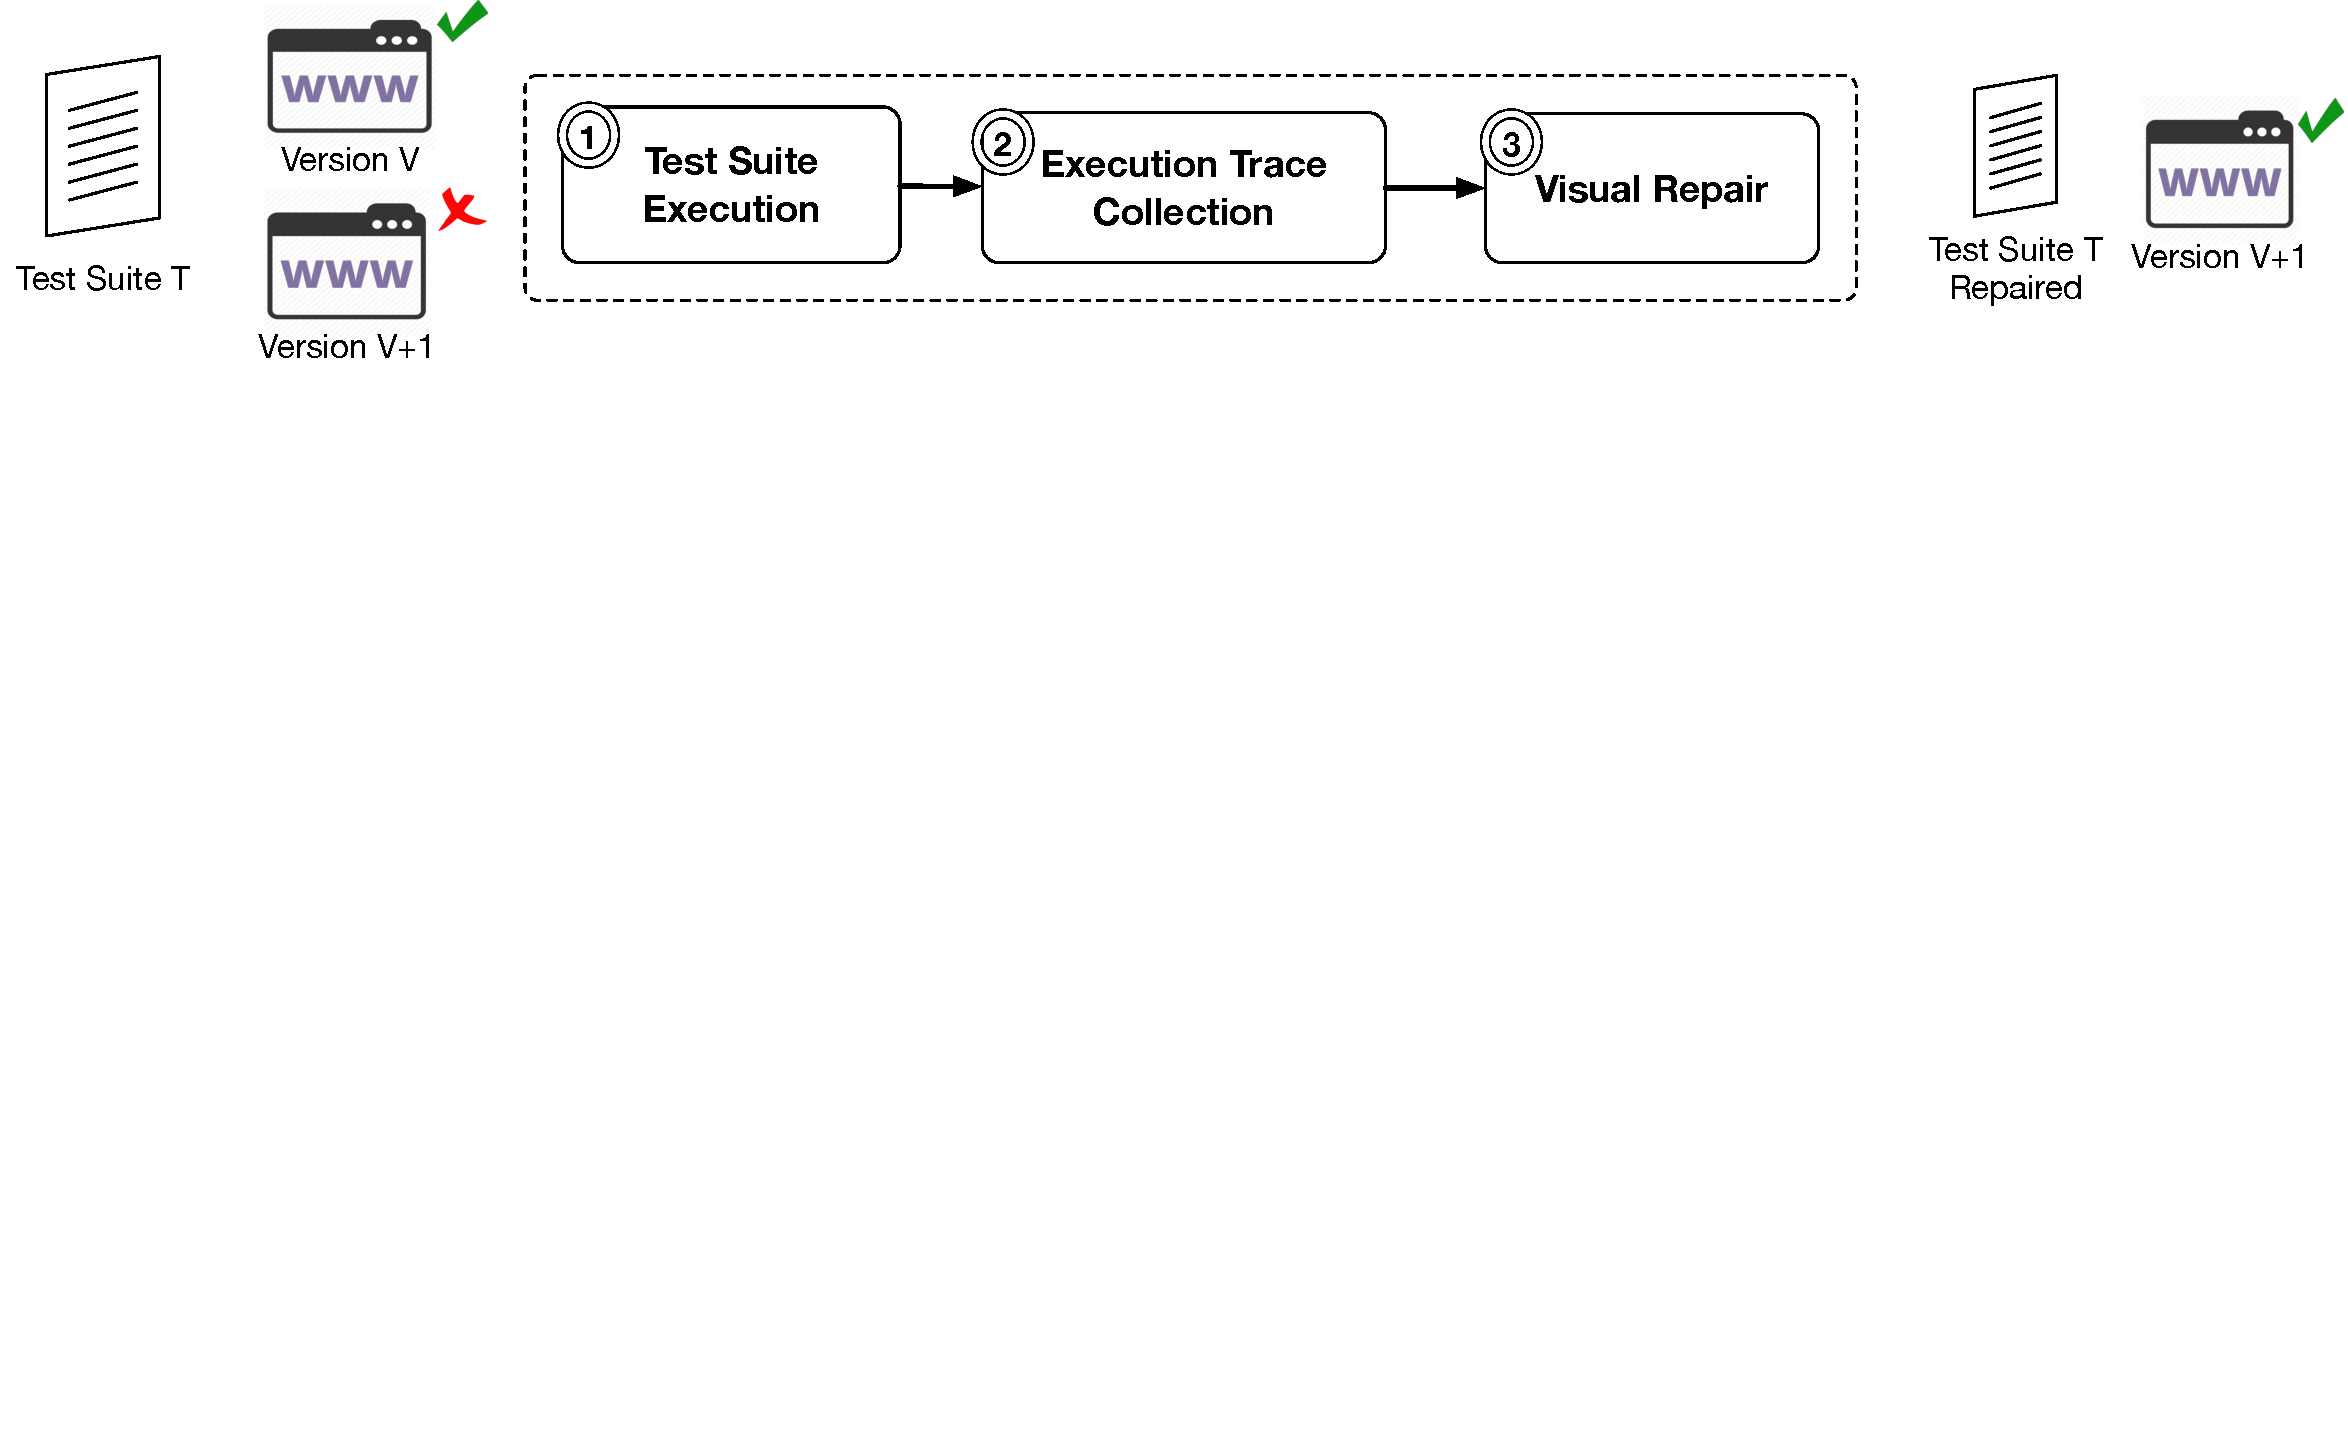
\includegraphics[trim={0.0cm 18cm 0.0cm 0cm},clip,scale=0.435]{images/approach-reduced2}
%}
\caption{High Level Overview of Visual Test Repair Approach}
\label{approach}
\end{figure*}


\subsubsection{Template Matching}

\begin{itemize}
\item use SIFT to determine whether the image is present/absent
\item SIFT returns also an estimate of where the majority of keypoints has been found
\item Template matching usually returns multiple or inaccurate results
\item the idea is to filter the TM results with SIFT's
\item one try might be to use multiple images (i.e. both the perfectly cropped and the larger visual locator).
\item try to implement Chamfer Matching
\end{itemize}

\subsubsection{Metrics}

\begin{enumerate}
\item The number of \textit{true positives} (TP):The number of samples that have been correctly identified as being the class being sought (e.g. that a face exists at a particular location).
\item The number of \textit{false positives} (FP): The number of samples that have been incorrectly identified as being the class being sought (e.g. that a face exists at a particular location when there is no face present).
\item The number of \textit{true negatives} (TN): The number of samples that have been correctly identified as not being the class being sought (e.g. that a face does not exist at a particular location).
\item The number of \textit{false negatives} (FN): The number of samples that have been incorrectly identified as not being the class being sought (e.g. that a face does not exist at a particular location when there is a face present at that location).
\item Recall is the percentage of the objects being sought which have been successfully located. Recall = TP / (TP + FN)
\item Precision is the percentage of the positive classifications which are correct (i.e. are not false alarms). Precision = TP / (TP + FP)
\item Accuracy is the percentage of the total samples which are correct. Accuracy = TP + TN / TotalSamples
\end{enumerate}






